\section{Results \& Discussion}

\subsection{Performance Metrics}
The purpose of this project is to assess the benefit of dynamic, or adaptive, thresholds-based algorithms over static ones (whether it be the homogeneous or heterogeneous case). To do so, we introduce two performance metrics, one being the number of tasks processed within a time period and the other one being the average distance traveled per processed task. While the former gives us an idea of the average rate at which actions are performed, the latter embeds two notions at the same time: the distribution of workload among robots and the efficiency of the allocation in terms of distance from robots to tasks.

   \begin{figure}[thpb]
      \centering
      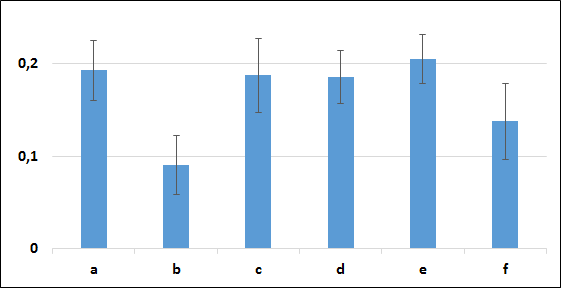
\includegraphics[width=8.5cm]{Pictures/PrivFixedMetric1.png}
      \caption{Number of events handled per time unit for the private, fixed-thresholds algorithms}
      \label{figure1}
   \end{figure}
	 \begin{figure}[thpb]
      \centering
      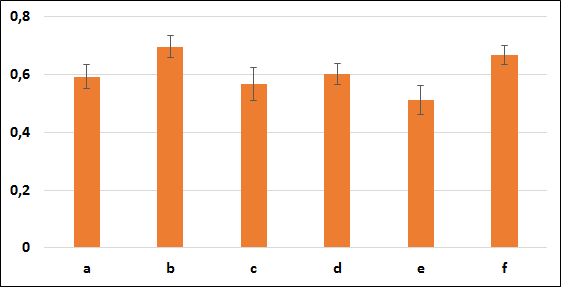
\includegraphics[width=8.5cm]{Pictures/PrivFixedMetric2.png}
      \caption{Distance traveled per event handled for the private, fixed-thresholds algorithms}
      \label{figure2}
   \end{figure}
	\begin{figure}[thpb]
      \centering
      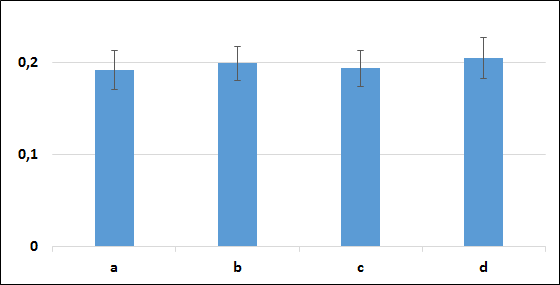
\includegraphics[width=8.5cm]{Pictures/PrivAdaptMetric1.png}
      \caption{Number of events handled per time unit for the private, adaptive-thresholds algorithms}
      \label{figure3}
   \end{figure}
	\begin{figure}[thpb]
      \centering
      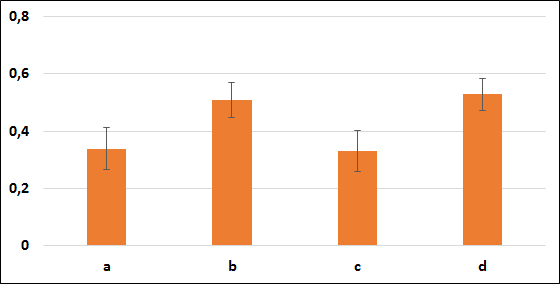
\includegraphics[width=8.5cm]{Pictures/PrivAdaptMetric2.png}
      \caption{Distance traveled per event handled for the private, adaptive-thresholds algorithms}
      \label{figure4}
   \end{figure}
	\begin{figure}[thpb]
      \centering
      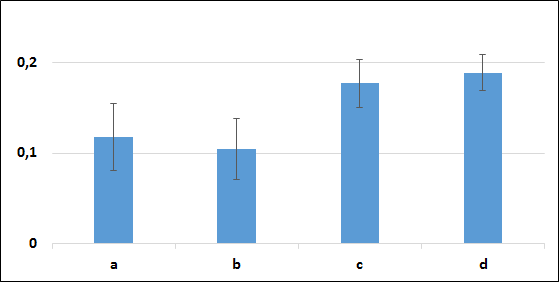
\includegraphics[width=8.5cm]{Pictures/PrivSpecMetric1.png}
      \caption{Number of events handled per time unit for the private, adaptive-thresholds with specialization algorithms}
      \label{figure5}
   \end{figure}
	\begin{figure}[thpb]
      \centering
      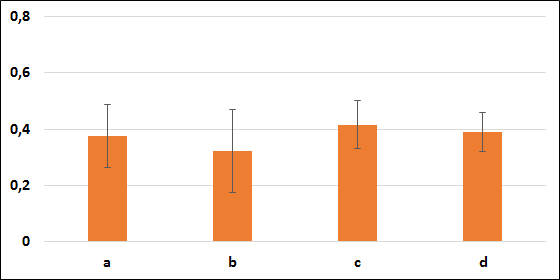
\includegraphics[width=8.5cm]{Pictures/PrivSpecMetric2.png}
      \caption{Distance traveled per event handled for the private, adaptive-thresholds with specialization algorithms}
      \label{figure6}
   \end{figure}
	\begin{figure}[thpb]
      \centering
      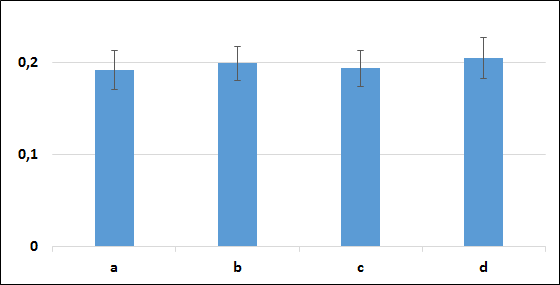
\includegraphics[width=8.5cm]{Pictures/PrivAdaptMetric1.png}
      \caption{Number of events handled per time unit for the public, adaptive-thresholds algorithms}
      \label{figure7}
   \end{figure}
	\begin{figure}[thpb]
      \centering
      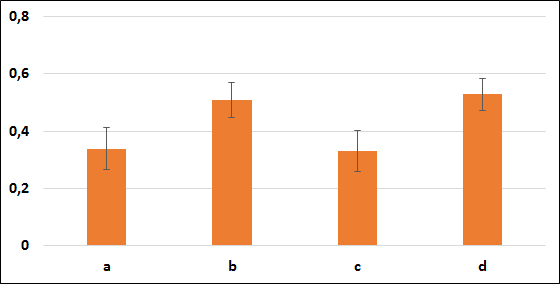
\includegraphics[width=8.5cm]{Pictures/PrivAdaptMetric2.png}
      \caption{Distance traveled per event handled for the public, adaptive-thresholds algorithms}
      \label{figure8}
   \end{figure}


[ EXPERIMENT 1: WE COULD TRY DIFFERENT THRESHOLD VALUES AND COMPARE PERFORMANCES | EXPERIMENT 2: WE COULD TRY DIFFERENT ADAPTATION MECHANISM (VISION OR TIME IN SEARCH MODE = COLORBLIND) AND COMPARE RESULTS | EXPERIMENT 3: WE COULD TRY DIFFERENT ADAPTATION FUNCTION FOR STIMULI AND COMPARE RESULTS | LAST PART: COMPARE ALL ALGORITHMS WITH BEST PERFORMANCE]